\documentclass[/home/jesse/Analysis/FemtoAnalysis/AnalysisNotes/AnalysisNoteJBuxton.tex]{subfiles}
\begin{document}

\section{Spherical Harmonics}
\label{Appendix_SphericalHarmonics}

This appendix shows a spherical harmonic decomposition of our \LamKs correlation functions.
For our purposes, the most interesting components are $C_{00}$ and $\Re C_{11}$, which are presented in Figures \ref{fig:LamKchP_ReC00C11_All} - \ref{fig:LamK0_ReC00C11_All}.
In each of the figures, the left column shows $C_{00}$, the right column $\Re C_{11}$, and the rows separate the centrality bins.
For the the 0-10\% bin, results are also included from a THERMINATOR 2 simulation for an impact parameter $b = $ 2 fm (gold stars) and assumed scattering parameters ($\Re f_{0}$, $\Im f_{0}$, $d_{0}$) = (-1.16, 0.51, 1.08), (0.41, 0.47, -4.89), and (-0.41, 0.20, 2.08) for the \LamKchP, \LamKchM, and \LamKs systems, respectively.
The coefficient $C_{00}$ quantifies the overall angle-integrated strength of the correlation function, similar to that studied in our 1D analysis.
The $\Re C_{11}$ term is sensitive to the asymmetry in the outward direction, a component interesting for non-identical particle studies.
In our analysis, we have taken the \Lam to be the first particle in our pairs, and a negative value of $\Re C_{11}$ signifies the \Lam particles are emitted, on average, further out and/or earlier than the K mesons.
For completeness, the first six components of the spherical harmonic decompositions are shown in Figures \ref{fig:LamKchP_FirstSixCYlm} - \ref{fig:LamK0_FirstSixCYlm}

\begin{figure}[h]
  \centering
  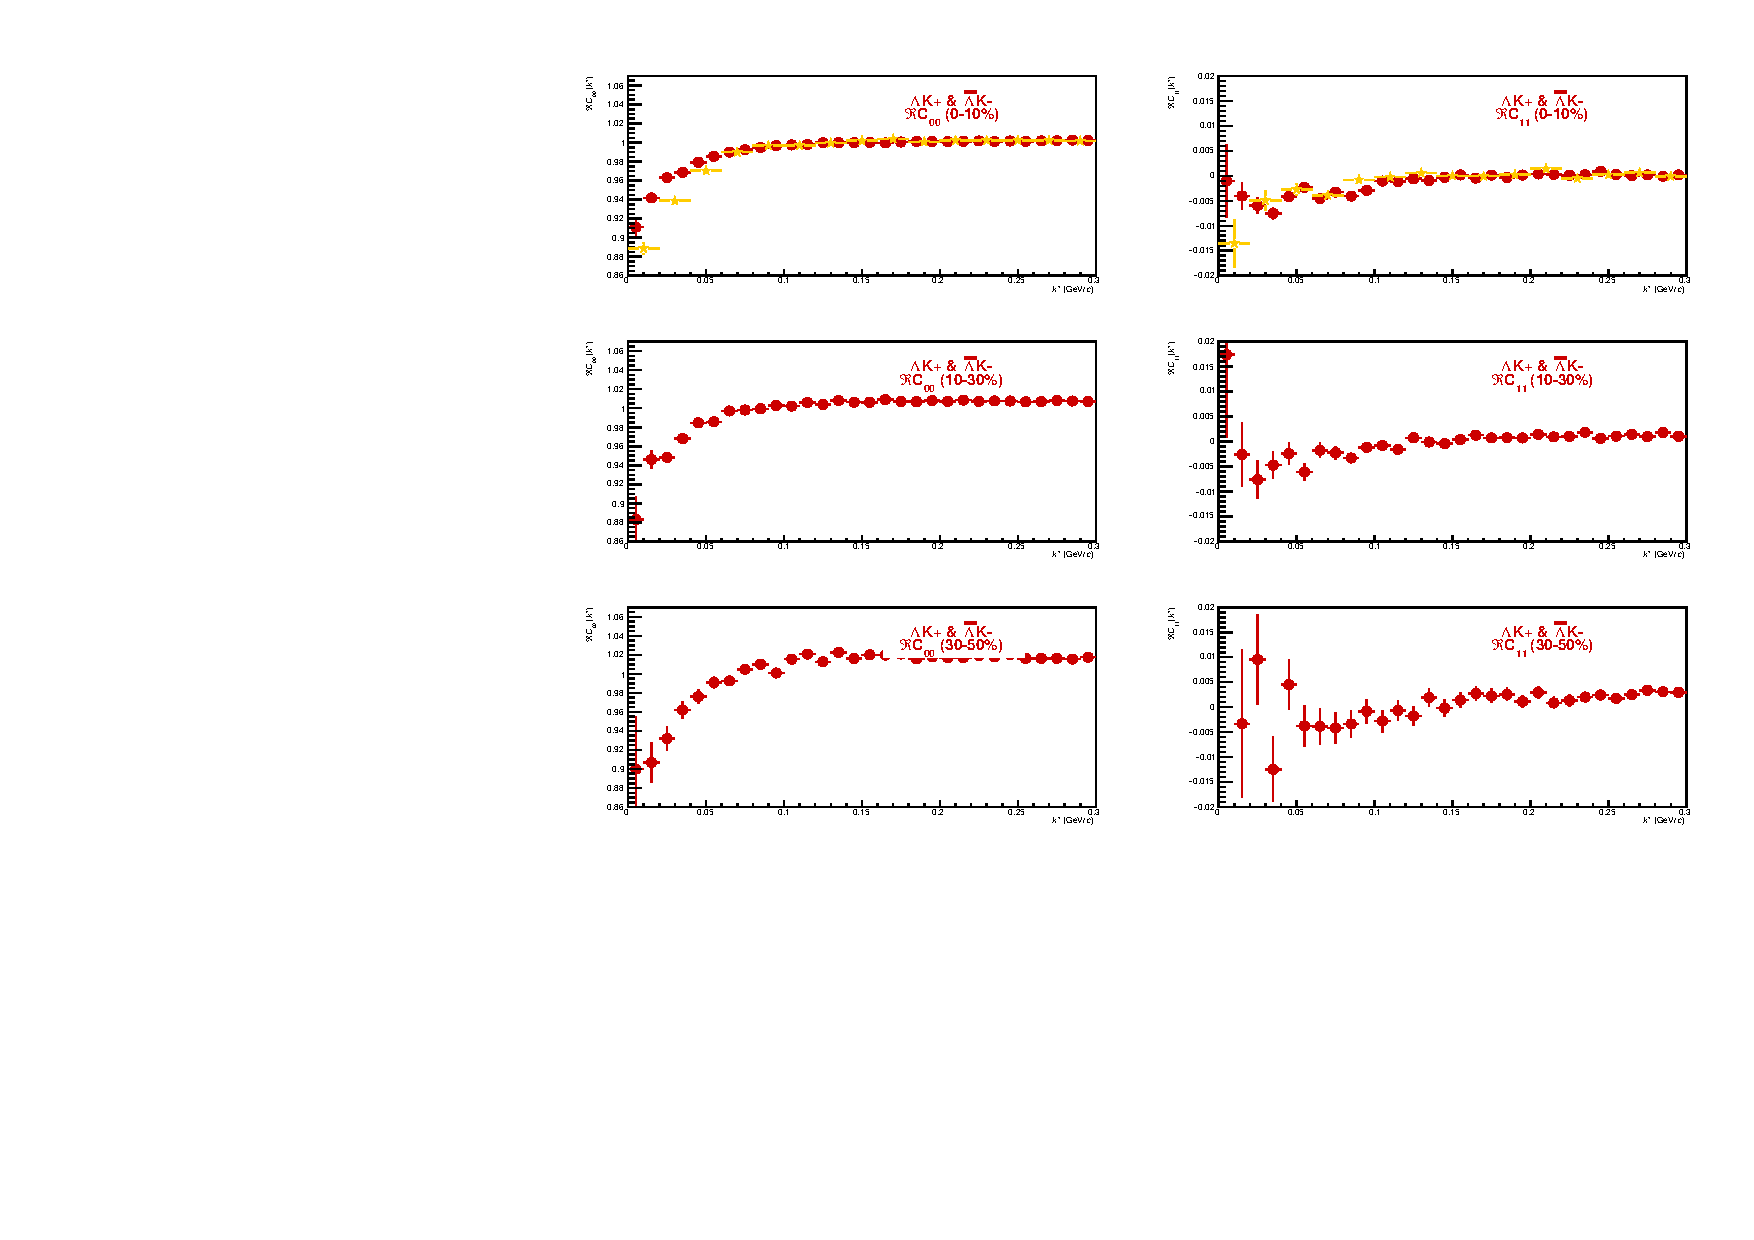
\includegraphics[width=\textwidth]{\ResultsDirBase Results_cLamcKch_20181205/SphericalHarmonics/LamKchP/CanCfYlmReC00C11_LamKchPALamKchM_All_wTherm.pdf}
  \caption[\LamKchP $C_{00}$ and $\Re C_{11}$ spherical harmonic components]
  {
  $C_{00}$ (left) and $\Re C_{11}$ (right) components of a spherical harmonic decomposition of the \LamKchP correlation function for the 0-10\% (top), 10-30\% (middle), and 30-50\% (bottom) centrality bins.
  For the the 0-10\% bin, results are also included from a THERMINATOR 2 simulation for an impact parameter $b = $ 2 fm (gold stars) and assumed scattering parameters ($\Re f_{0}$, $\Im f_{0}$, $d_{0}$) = (-1.16, 0.51, 1.08).
  }
  \label{fig:LamKchP_ReC00C11_All}
\end{figure}


\begin{figure}[h]
  \centering
  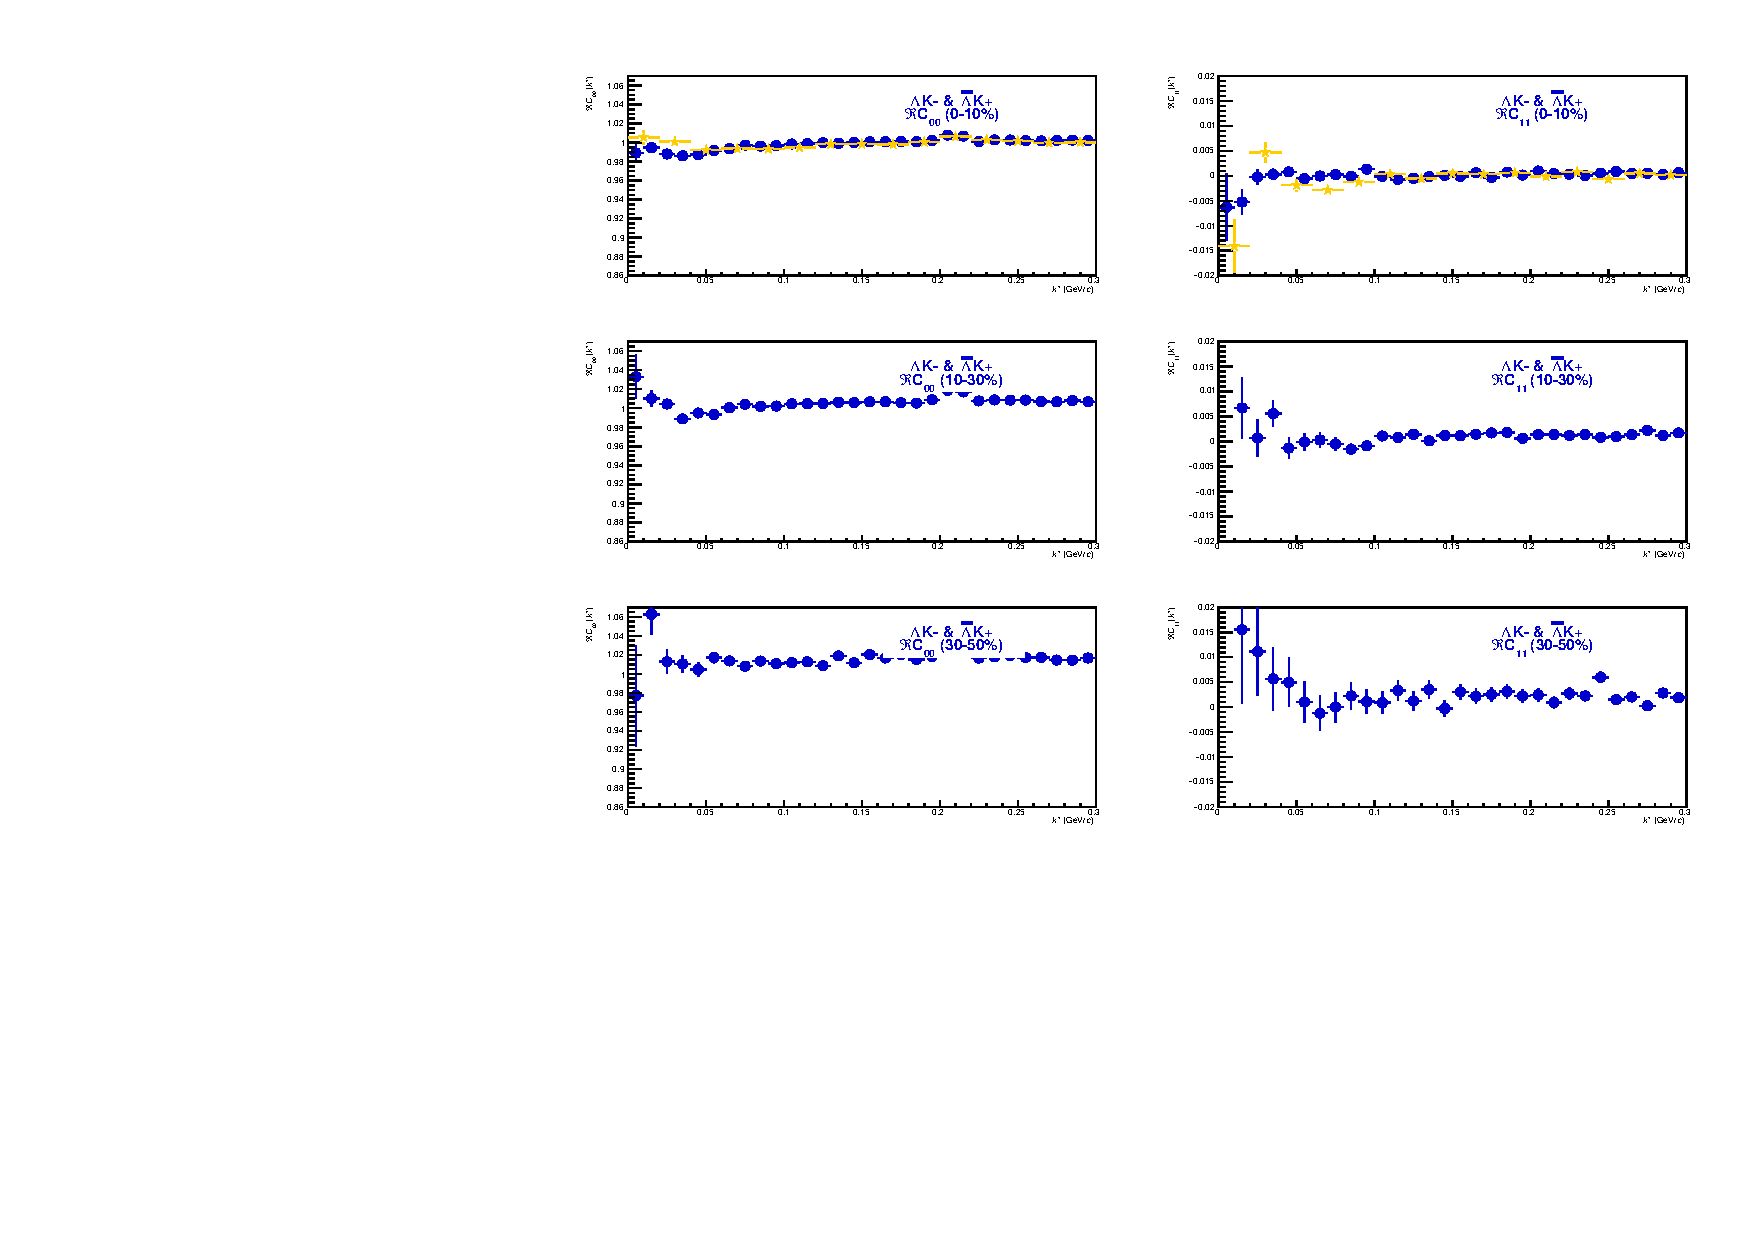
\includegraphics[width=\textwidth]{\ResultsDirBase Results_cLamcKch_20181205/SphericalHarmonics/LamKchM/CanCfYlmReC00C11_LamKchMALamKchP_All_wTherm.pdf}
  \caption[\LamKchM $C_{00}$ and $\Re C_{11}$ spherical harmonic components]
  {
  $C_{00}$ (left) and $\Re C_{11}$ (right) components of a spherical harmonic decomposition of the \LamKchM correlation function for the 0-10\% (top), 10-30\% (middle), and 30-50\% (bottom) centrality bins.
  For the the 0-10\% bin, results are also included from a THERMINATOR 2 simulation for an impact parameter $b = $ 2 fm (gold stars) and assumed scattering parameters ($\Re f_{0}$, $\Im f_{0}$, $d_{0}$) = (0.41, 0.47, -4.89).
  }
  \label{fig:LamKchM_ReC00C11_All}
\end{figure}

\begin{figure}[h]
  \centering
  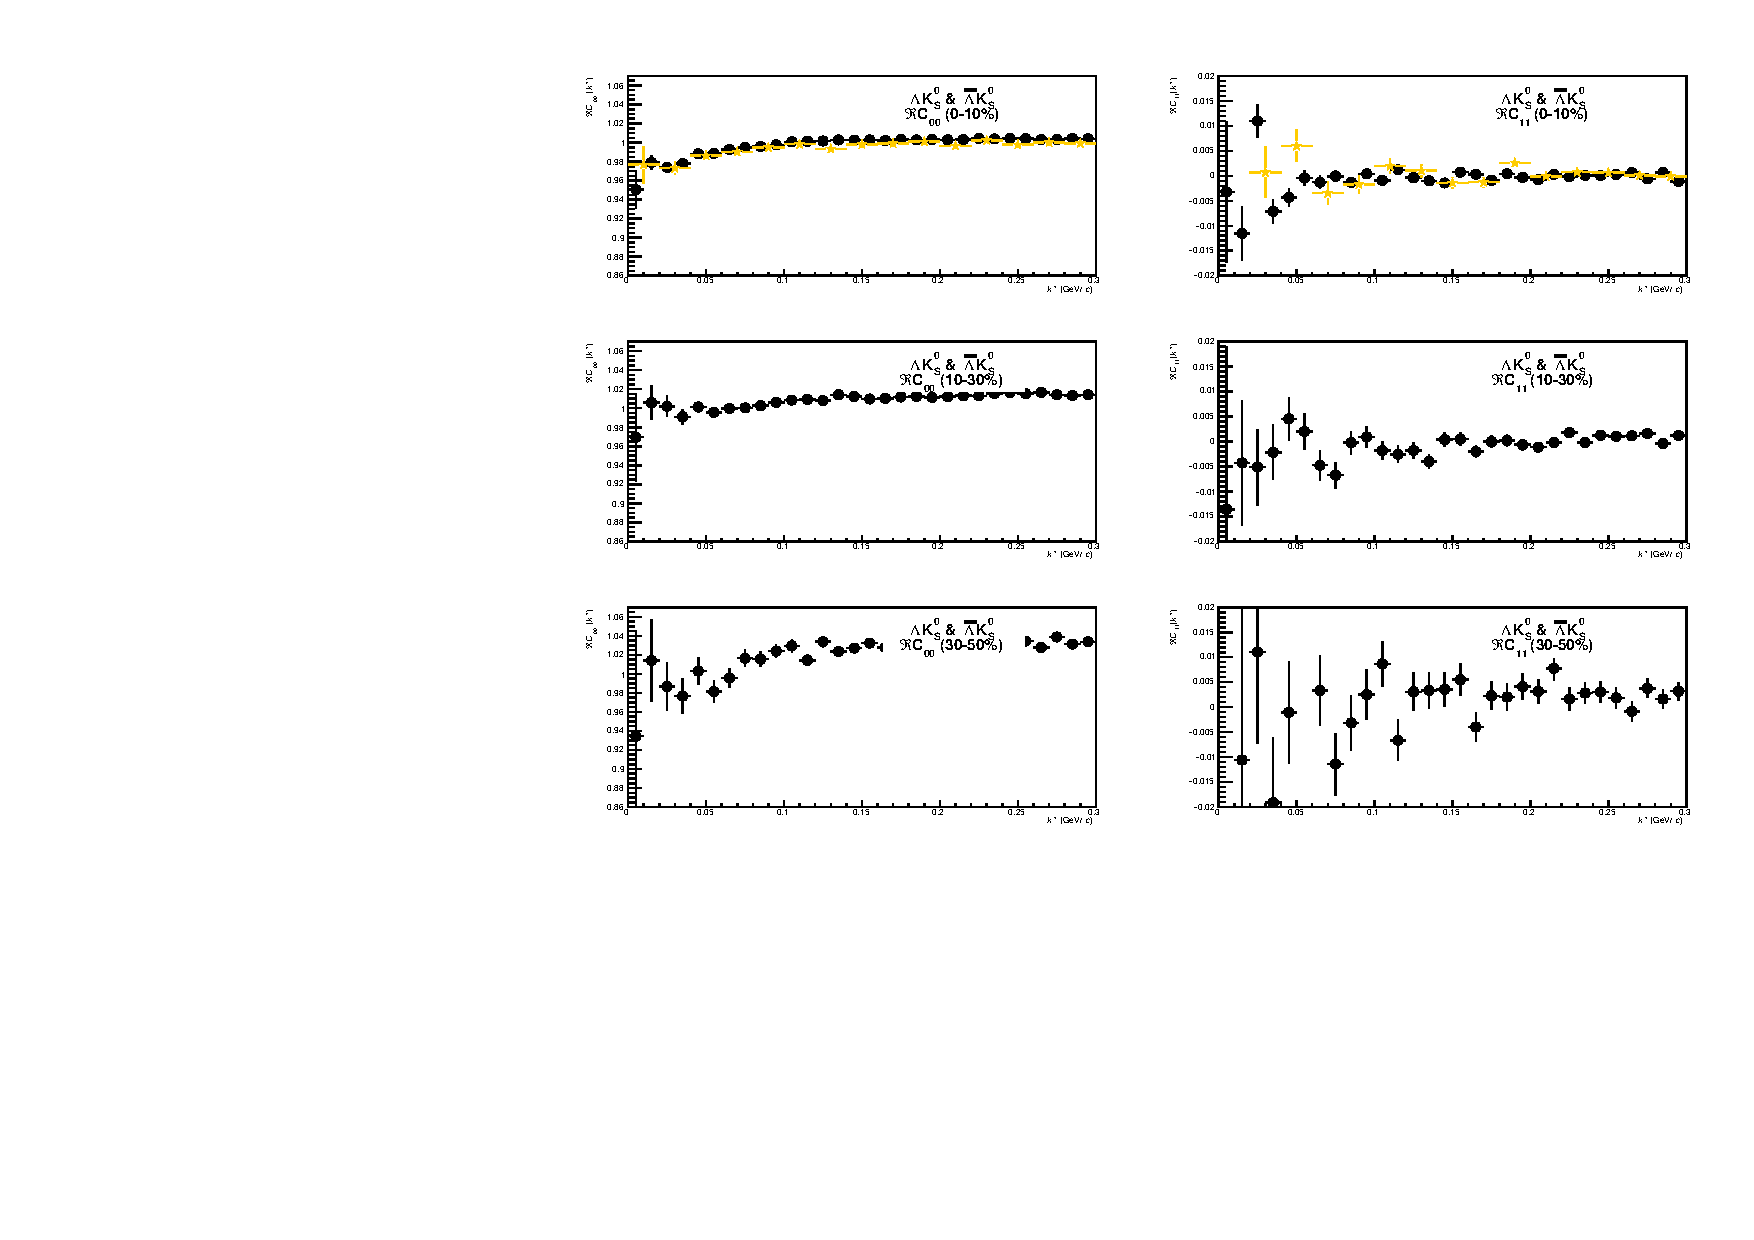
\includegraphics[width=\textwidth]{\ResultsDirBase Results_cLamK0_20181205/SphericalHarmonics/LamK0/CanCfYlmReC00C11_LamK0ALamK0_All_wTherm.pdf}
  \caption[\LamKs $C_{00}$ and $\Re C_{11}$ spherical harmonic components]
  {
  $C_{00}$ (left) and $\Re C_{11}$ (right) components of a spherical harmonic decomposition of the \LamKs correlation function for the 0-10\% (top), 10-30\% (middle), and 30-50\% (bottom) centrality bins.
  For the the 0-10\% bin, results are also included from a THERMINATOR 2 simulation for an impact parameter $b = $ 2 fm (gold stars) and assumed scattering parameters ($\Re f_{0}$, $\Im f_{0}$, $d_{0}$) = (-0.41, 0.20, 2.08).
  }
  \label{fig:LamK0_ReC00C11_All}
\end{figure}



\begin{figure}[h!]
  \centering
  %%----start of first subfigure---  
  \subfloat[Real components, $\Re C_{lm}$]{
    \label{fig:LamKchP_FirstSixCYlm:a}
    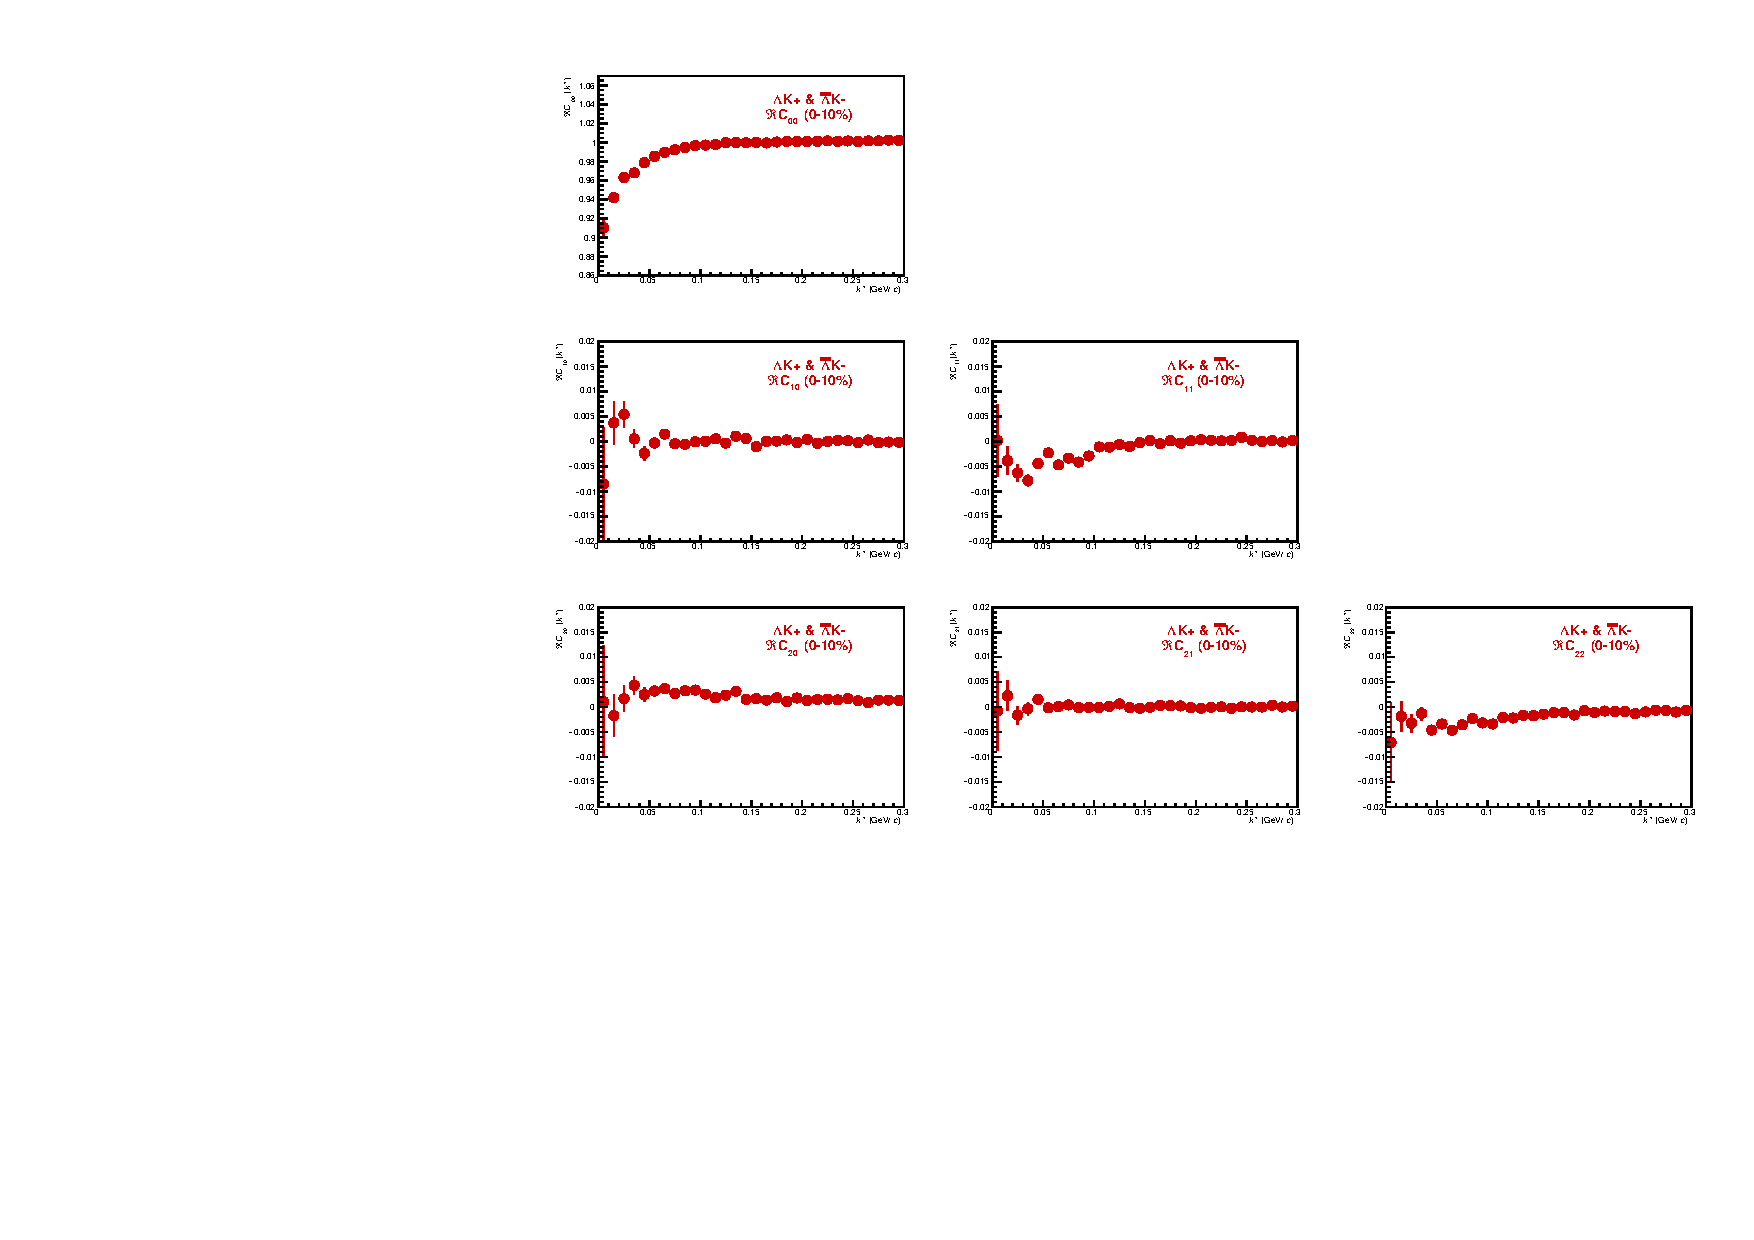
\includegraphics[width=0.9\linewidth]{\ResultsDirBase Results_cLamcKch_20181205/SphericalHarmonics/LamKchP/CanCfYlmReFirstSixComps_LamKchPALamKchM_0010.pdf}} \\
  %%----start of second subfigure---
  \subfloat[Imaginary components, $\Im C_{lm}$]{
    \label{fig:LamKchP_FirstSixCYlm:b}
    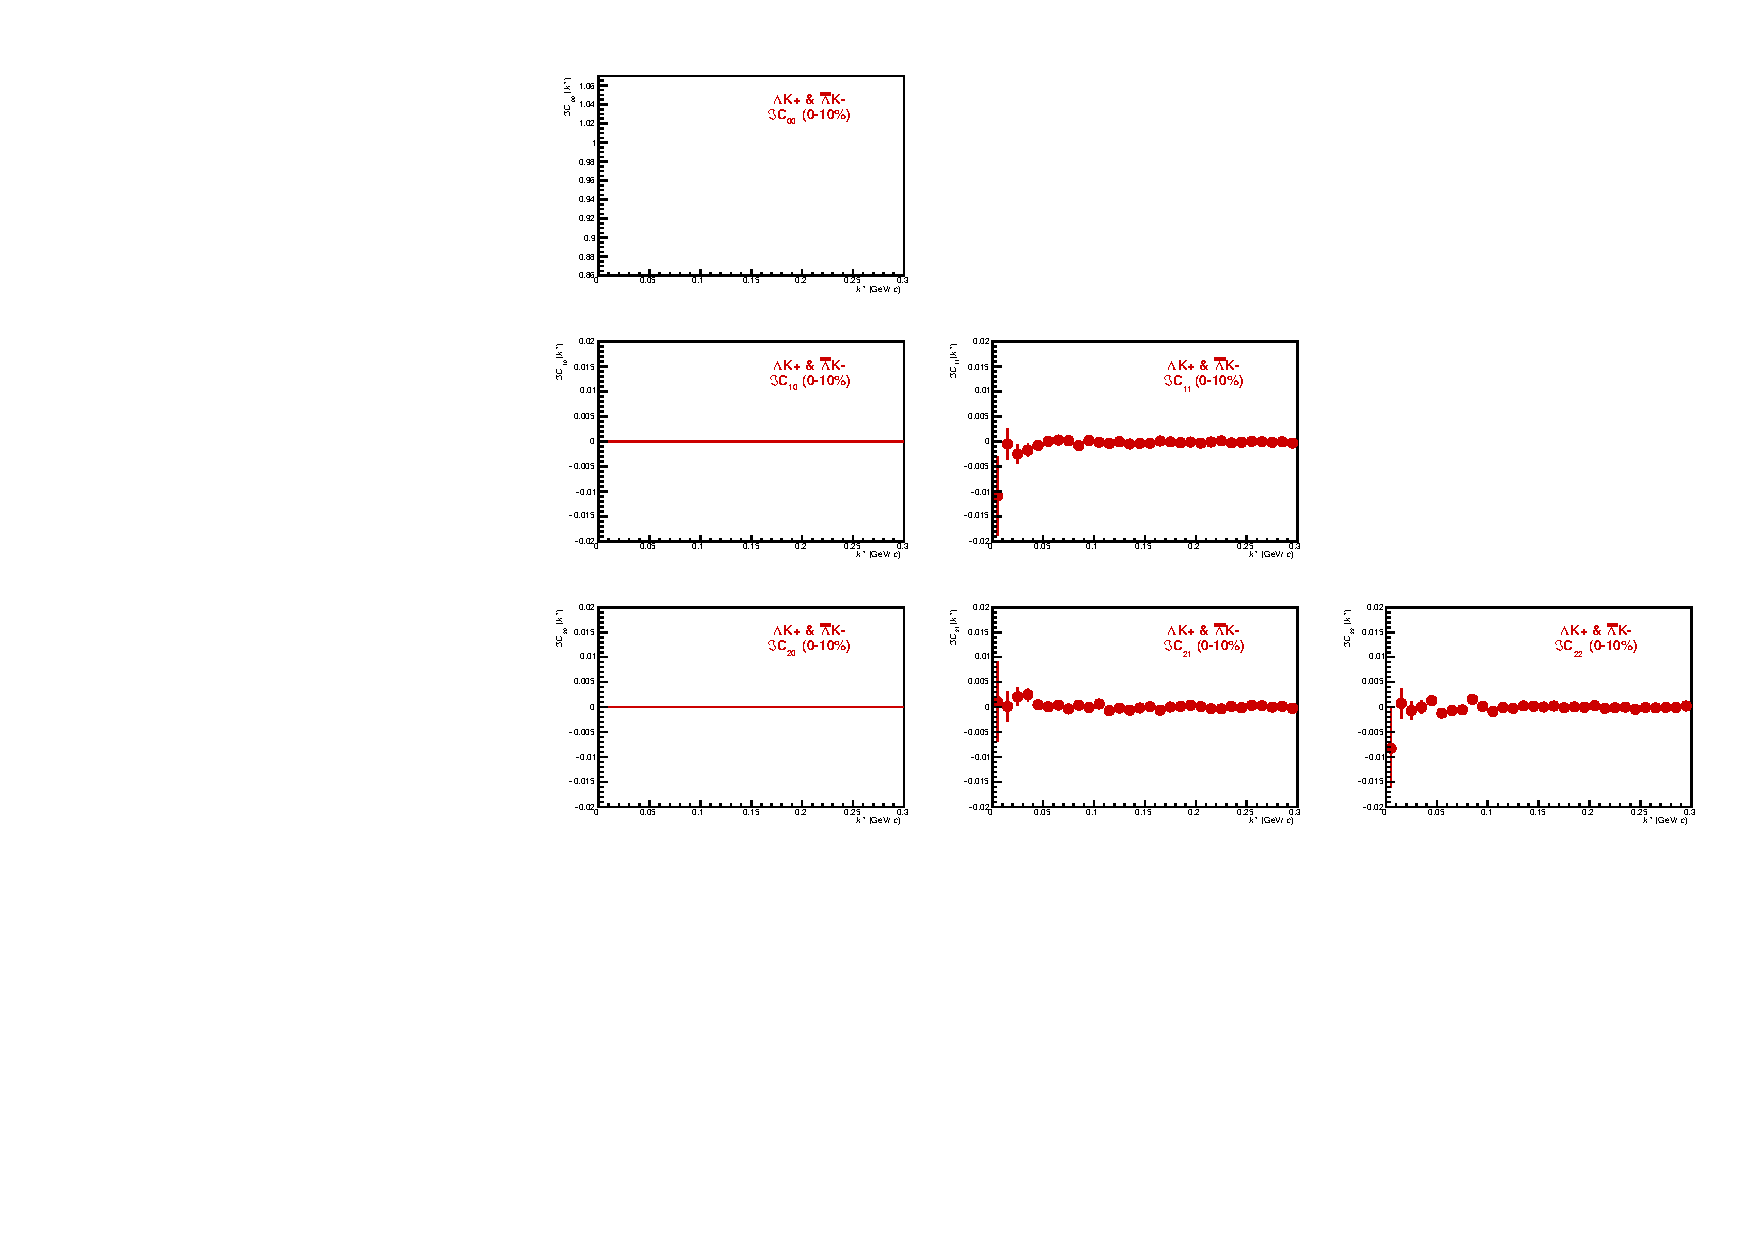
\includegraphics[width=0.9\linewidth]{\ResultsDirBase Results_cLamcKch_20181205/SphericalHarmonics/LamKchP/CanCfYlmImFirstSixComps_LamKchPALamKchM_0010.pdf}}  
  %%----overall caption----
  \caption[\LamKchP first six components of SH decomposition (0-10\%)]
  {
  First six components ($C_{00}, C_{10}, C_{11}, C_{20}, C_{21}, C_{22}$) of the spherical harmonic decomposition of the \LamKchP correlation function for the 0-10\% centrality bin.
  Note, $\Im C_{00}$, $\Im C_{10}$, and $\Im C_{20}$ are zero by definition.
  
  }
  \label{fig:LamKchP_FirstSixCYlm}
\end{figure}






\begin{figure}[h!]
  \centering
  %%----start of first subfigure---  
  \subfloat[Real components, $\Re C_{lm}$]{
    \label{fig:LamKchM_FirstSixCYlm:a}
    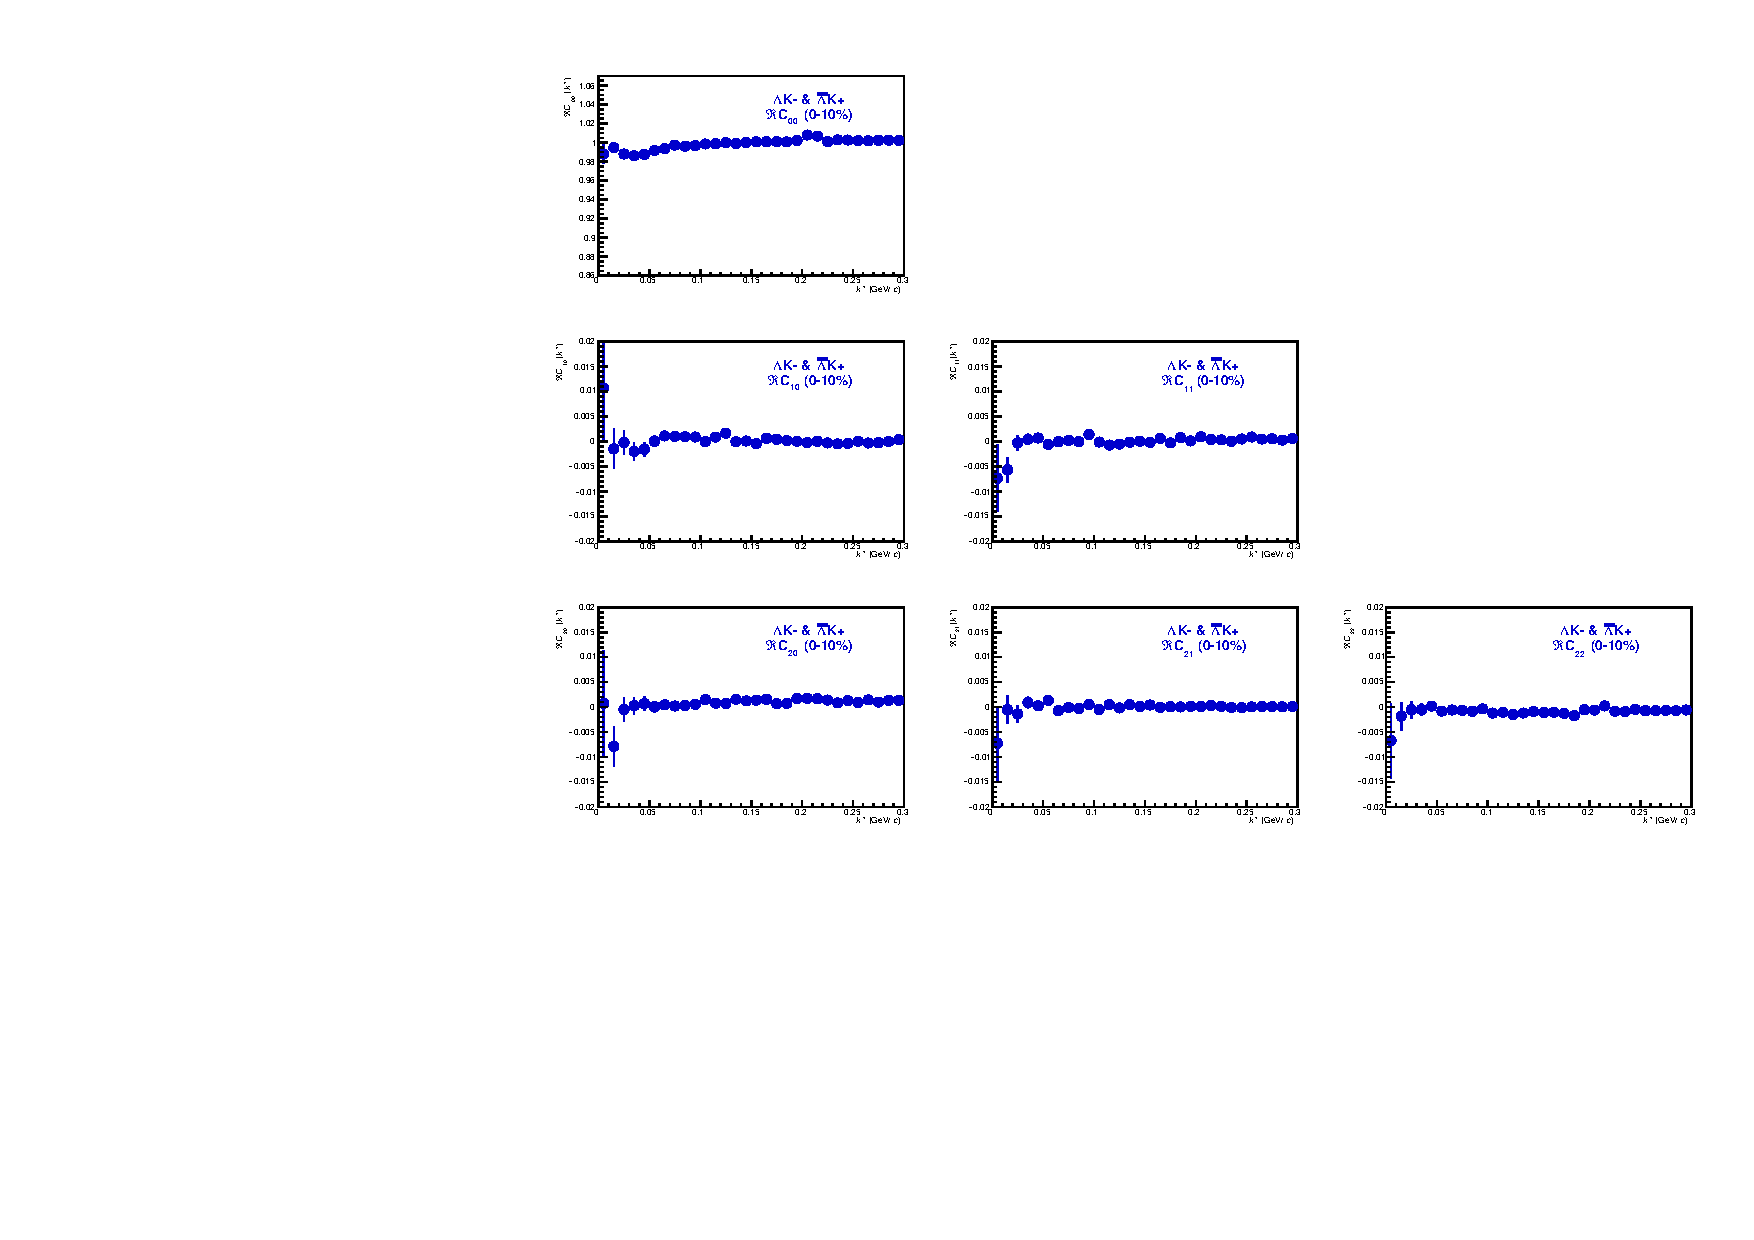
\includegraphics[width=0.9\linewidth]{\ResultsDirBase Results_cLamcKch_20181205/SphericalHarmonics/LamKchM/CanCfYlmReFirstSixComps_LamKchMALamKchP_0010.pdf}} \\
  %%----start of second subfigure---
  \subfloat[Imaginary components, $\Im C_{lm}$]{
    \label{fig:LamKchM_FirstSixCYlm:b}
    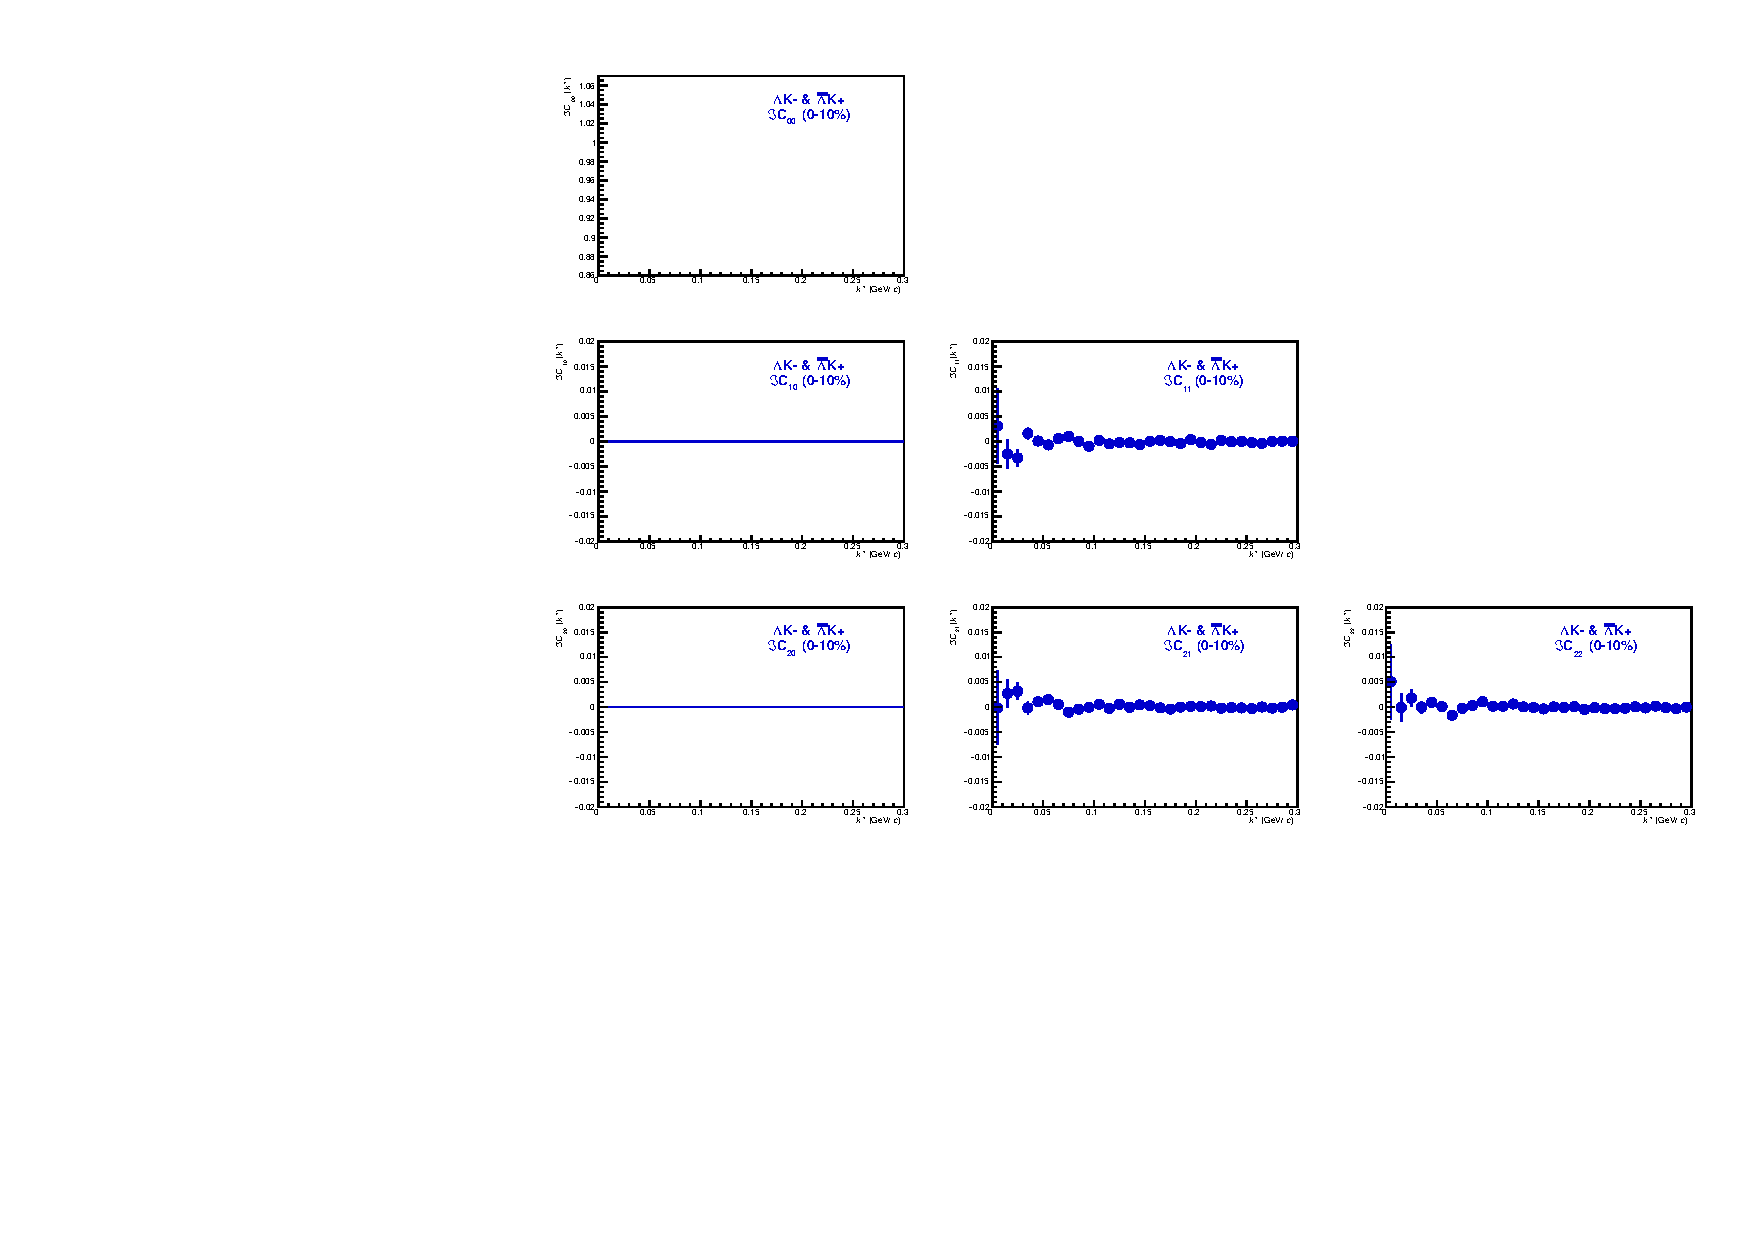
\includegraphics[width=0.9\linewidth]{\ResultsDirBase Results_cLamcKch_20181205/SphericalHarmonics/LamKchM/CanCfYlmImFirstSixComps_LamKchMALamKchP_0010.pdf}}  
  %%----overall caption----
  \caption[\LamKchM first six components of SH decomposition (0-10\%)]
  {
  First six components ($C_{00}, C_{10}, C_{11}, C_{20}, C_{21}, C_{22}$) of the spherical harmonic decomposition of the \LamKchM correlation function for the 0-10\% centrality bin.
  Note, $\Im C_{00}$, $\Im C_{10}$, and $\Im C_{20}$ are zero by definition.
  }
  \label{fig:LamKchM_FirstSixCYlm}
\end{figure}



\begin{figure}[h!]
  \centering
  %%----start of first subfigure---  
  \subfloat[Real components, $\Re C_{lm}$]{
    \label{fig:LamK0_FirstSixCYlm:a}
    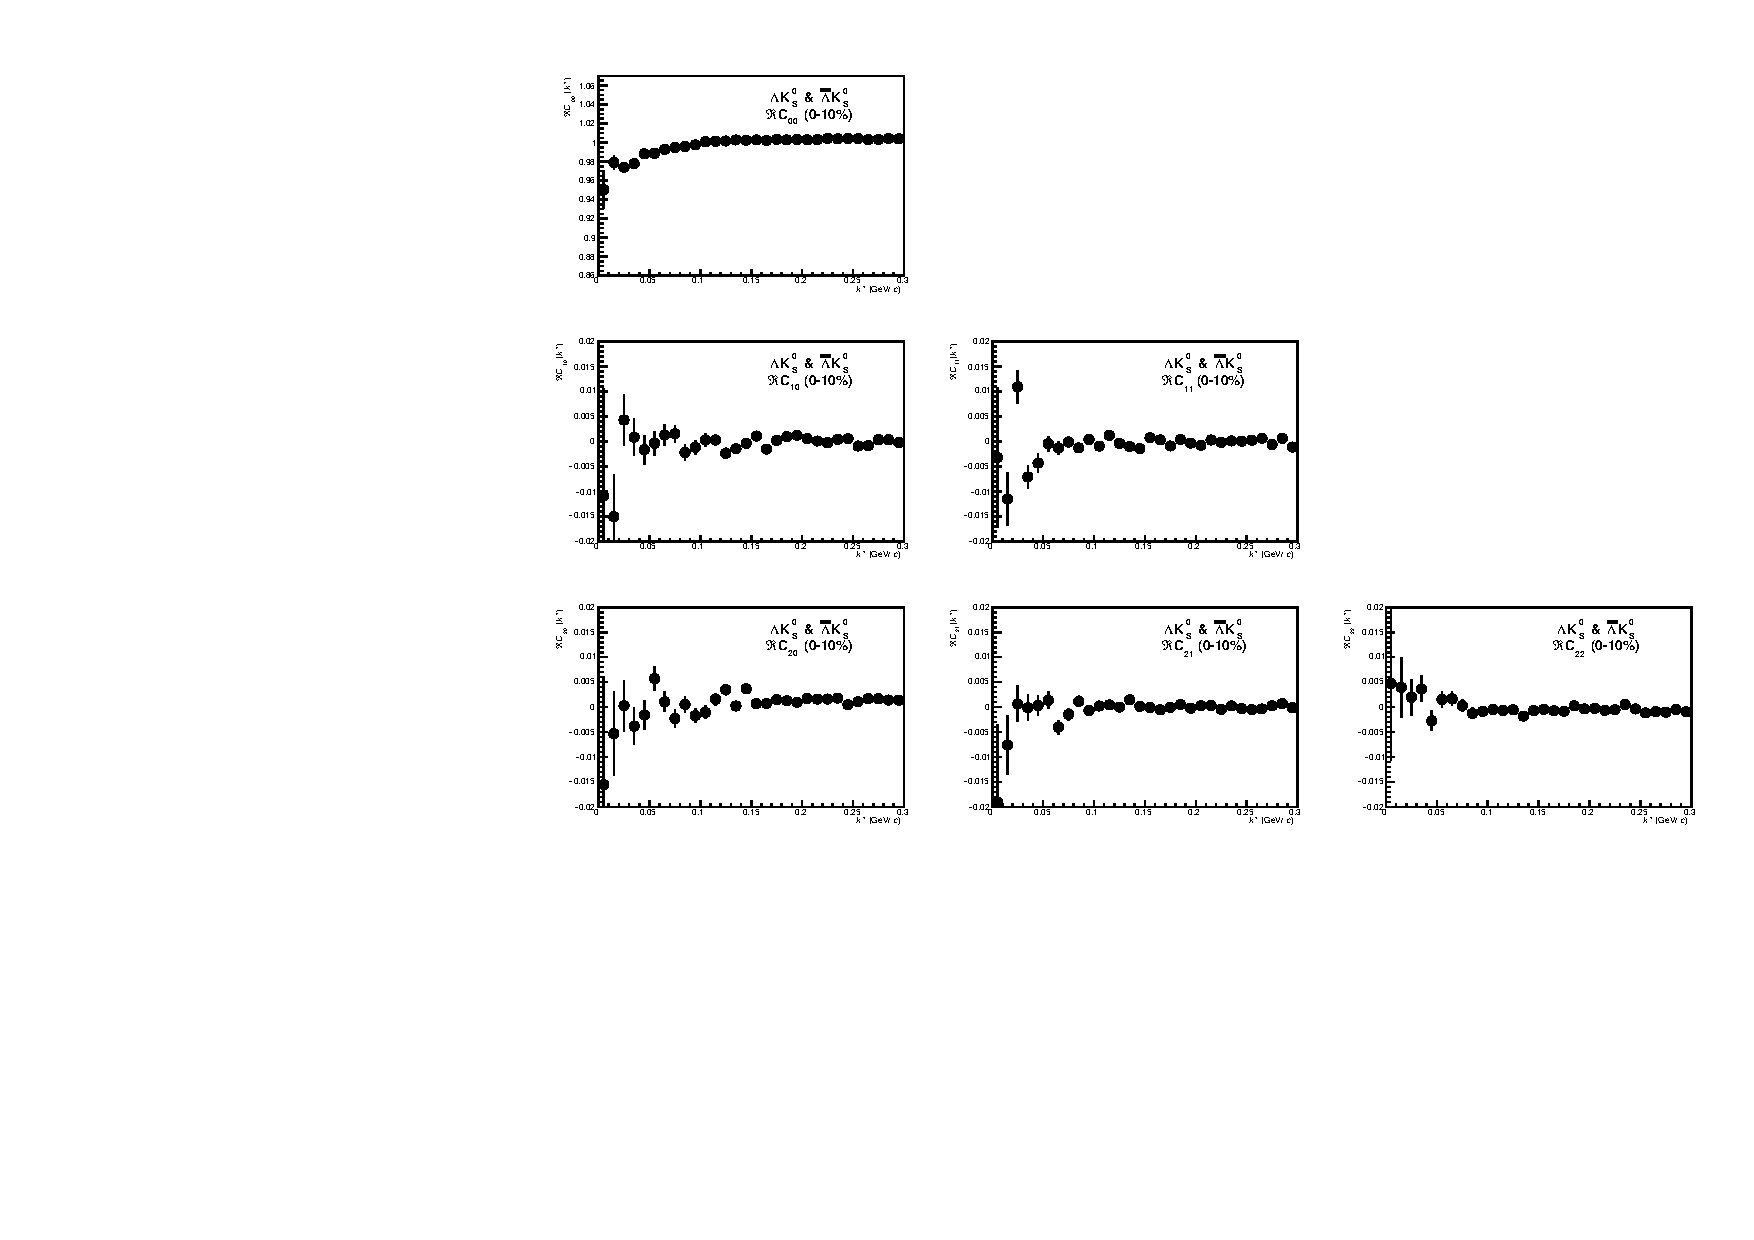
\includegraphics[width=0.9\linewidth]{\ResultsDirBase Results_cLamK0_20181205/SphericalHarmonics/LamK0/CanCfYlmReFirstSixComps_LamK0ALamK0_0010.pdf}} \\
  %%----start of second subfigure---
  \subfloat[Imaginary components, $\Im C_{lm}$]{
    \label{fig:LamK0_FirstSixCYlm:b}
    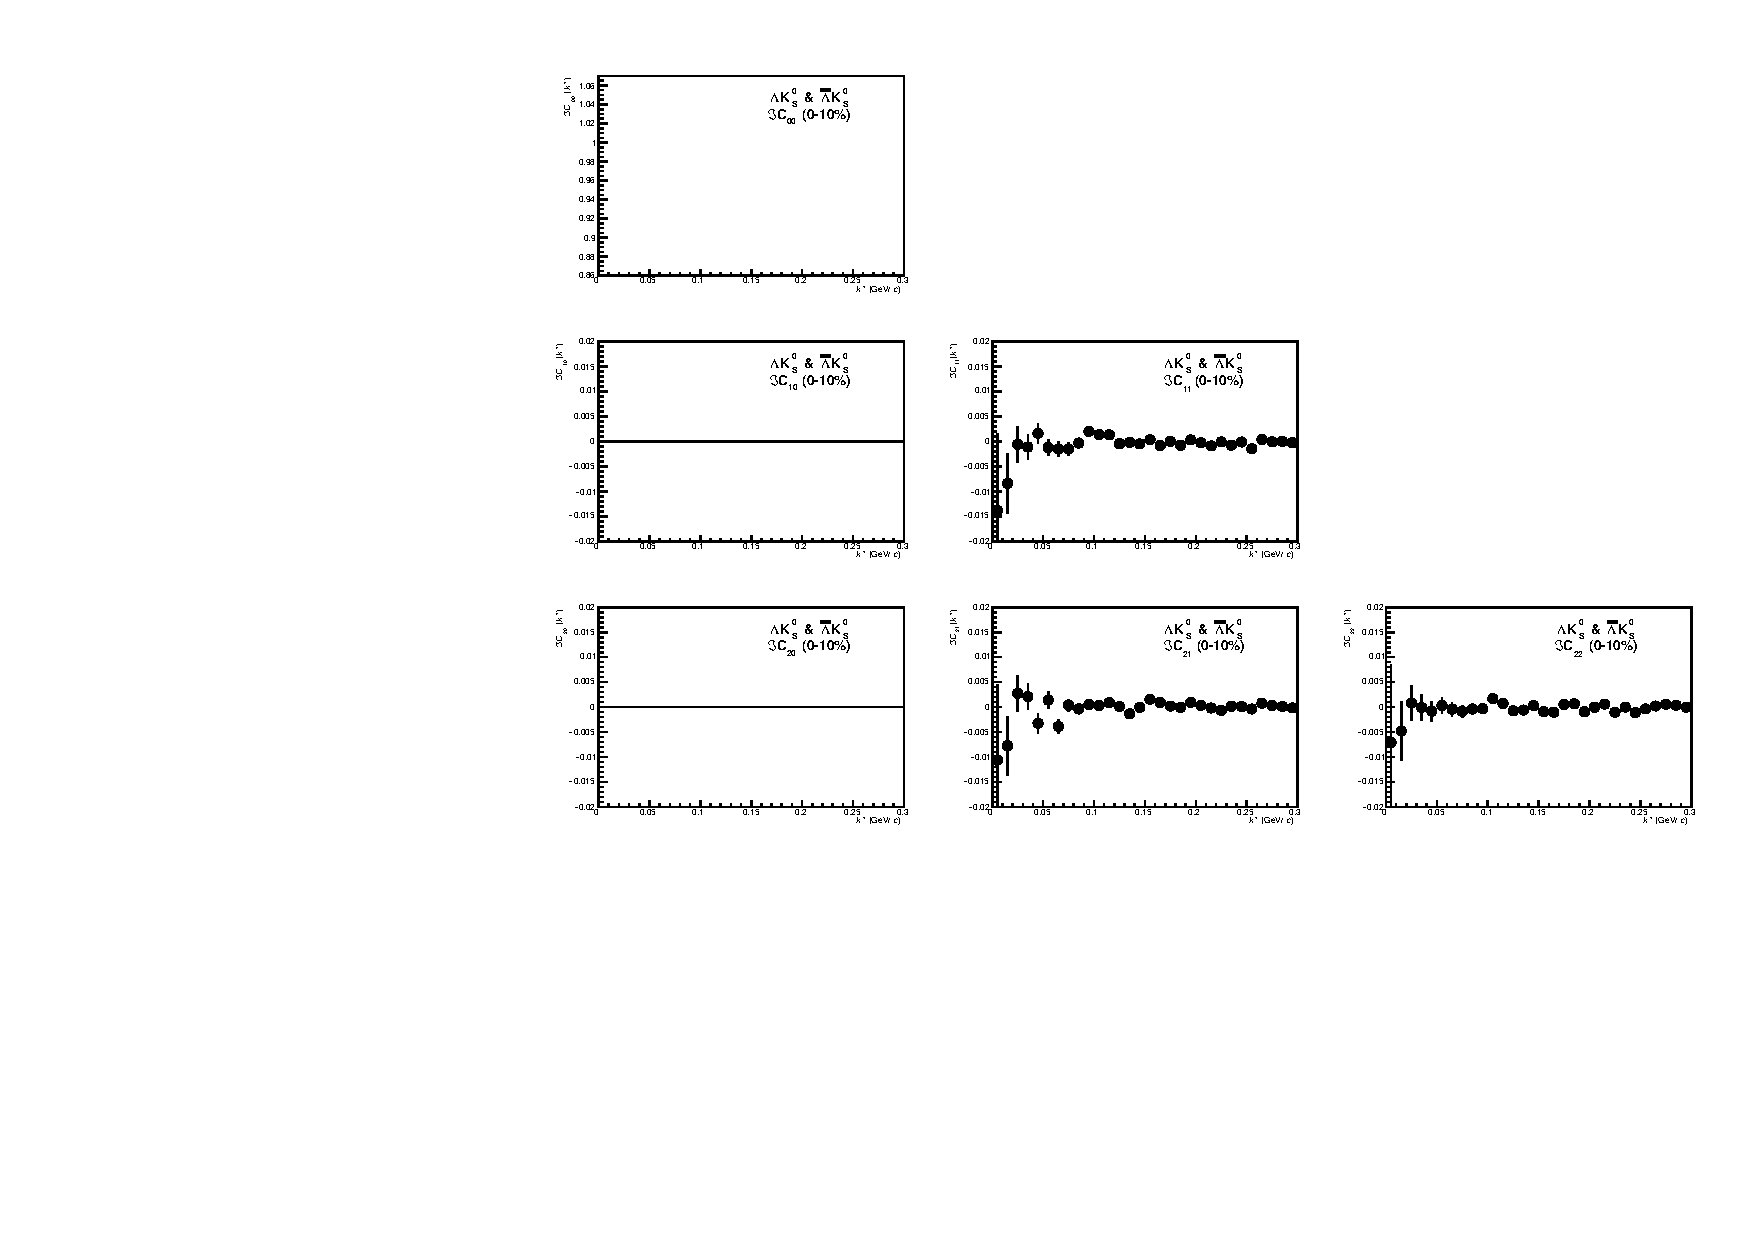
\includegraphics[width=0.9\linewidth]{\ResultsDirBase Results_cLamK0_20181205/SphericalHarmonics/LamK0/CanCfYlmImFirstSixComps_LamK0ALamK0_0010.pdf}}  
  %%----overall caption----
  \caption[\LamKs first six components of SH decomposition (0-10\%)]
  {
  First six components ($C_{00}, C_{10}, C_{11}, C_{20}, C_{21}, C_{22}$) of the spherical harmonic decomposition of the \LamKs correlation function for the 0-10\% centrality bin.
  Note, $\Im C_{00}$, $\Im C_{10}$, and $\Im C_{20}$ are zero by definition.
  }
  \label{fig:LamK0_FirstSixCYlm}
\end{figure}

\clearpage

\end{document}